\documentclass[11pt]{article}
\usepackage[french]{babel}
\usepackage{geometry}
\geometry{hmargin=2cm,vmargin=2cm}
\usepackage{eucal}
\usepackage{colortbl}
\usepackage{lscape}
\usepackage{amssymb}
\usepackage{amscd} 
\usepackage{fontspec} 
\usepackage{amsfonts,amsmath,amsthm,amssymb,stmaryrd,eurosym} 
\usepackage{textcomp}
\usepackage{icomma}
\usepackage{calrsfs}
\usepackage{fancyhdr}
\usepackage{makecell}
\usepackage{graphicx}
\renewcommand{\v}[1]{\overrightarrow{#1}}
\usepackage[svgnames,dvipsnames]{xcolor}
\newcommand{\fboxb}[1]{\fbox{\color{blue}#1\color{black}}}
\renewcommand{\b}[0]{$\bullet$}
\usepackage{tcolorbox}
\newcommand{\boite}[4]{\begin{tcolorbox}[colback=#1%couleur de fond
,colframe=#2 % couleur de bordure
,title= \begin{Large} %titre
	#3\end{Large}]
	#4 %contenu
	\end{tcolorbox}}





\title{Projet Pluridisciplinaire d'Informatique Intégrative}
\author{BEKHEDDA Maxence, GERMAIN Léo, GIANELLI Thomas, WALTER Théo}
\date{\today}
\begin{document}
\thispagestyle{empty}
\vspace*{-1.5cm}

\hspace{-1.5cm}
\includegraphics[scale=0.2]{logo_tn.jpg}
	
\vspace*{-1.6cm}
	
\hspace{13.5cm}
\includegraphics[scale=0.2]{logo_ul.png}



\vspace*{5cm}	% Espacement vertical
\begin{center}	% On centre le texte
{\huge \bf Projet Pluridisciplinaire d'Informatique Intégrative}\\	% \huge fait que le texte est gros, \bf fait que le texte est gras
\vspace{3cm}
\Large Recherche de solutions innovantes dans les circuits courts et les jardins partagés\\
\vspace{3cm}
Travail réalisé par BEKHEDDA Maxence,
GERMAIN Léo, \\GIANELLI Thomas et WALTER Théo
\vfill	% On va jusqu'au bas de la page avant de mettre le texte ci-dessous
\today
\end{center}
\newpage


\tableofcontents
\newpage


\section{Introduction}

Face au grand défi du XXIe siècle, le réchauffement climatique, les Hommes doivent remettre en question leur mode de vie. Cela passe notamment par leur manière de consommer. C’est pourquoi le gouvernement français a réalisé plusieurs actions récentes (comme avec le plan France Relance établi en 2020) afin d’inciter les consommateurs à davantage produire et consommer en circuit-court. Cette démarche de circuit-court vise à réduire au maximum le nombre d’intermédiaires entre le producteur et le consommateur. Cela permet de réduire le bilan carbone dû à la transportation du produit, contribuant donc à adopter un mode de consommation plus respectueux de l’environnement. De plus, cela permet de rémunérer justement les producteurs locaux et de leur permettre de prospérer. 
\vspace{0.2cm}

Dans le cadre de notre projet, nous souhaitons étendre cette démarche non seulement aux agriculteurs, mais également aux particuliers produisant des fruits et légumes transformés ou non. 
\section{État de l'art}

\subsection{Les casiers automatiques et les distributeurs de produits fermiers}

Ces dispositifs existent déjà depuis une vingtaine d'années en Allemagne et se démocratisent peu à peu en France. Les producteurs disposent dans des casiers, réfrigérés ou non, leurs produits que les clients vont ensuite pouvoir acheter. Après avoir payer sur la borne automatique, le casier choisi s'ouvre et le client récupère sa commande.

\begin{center}
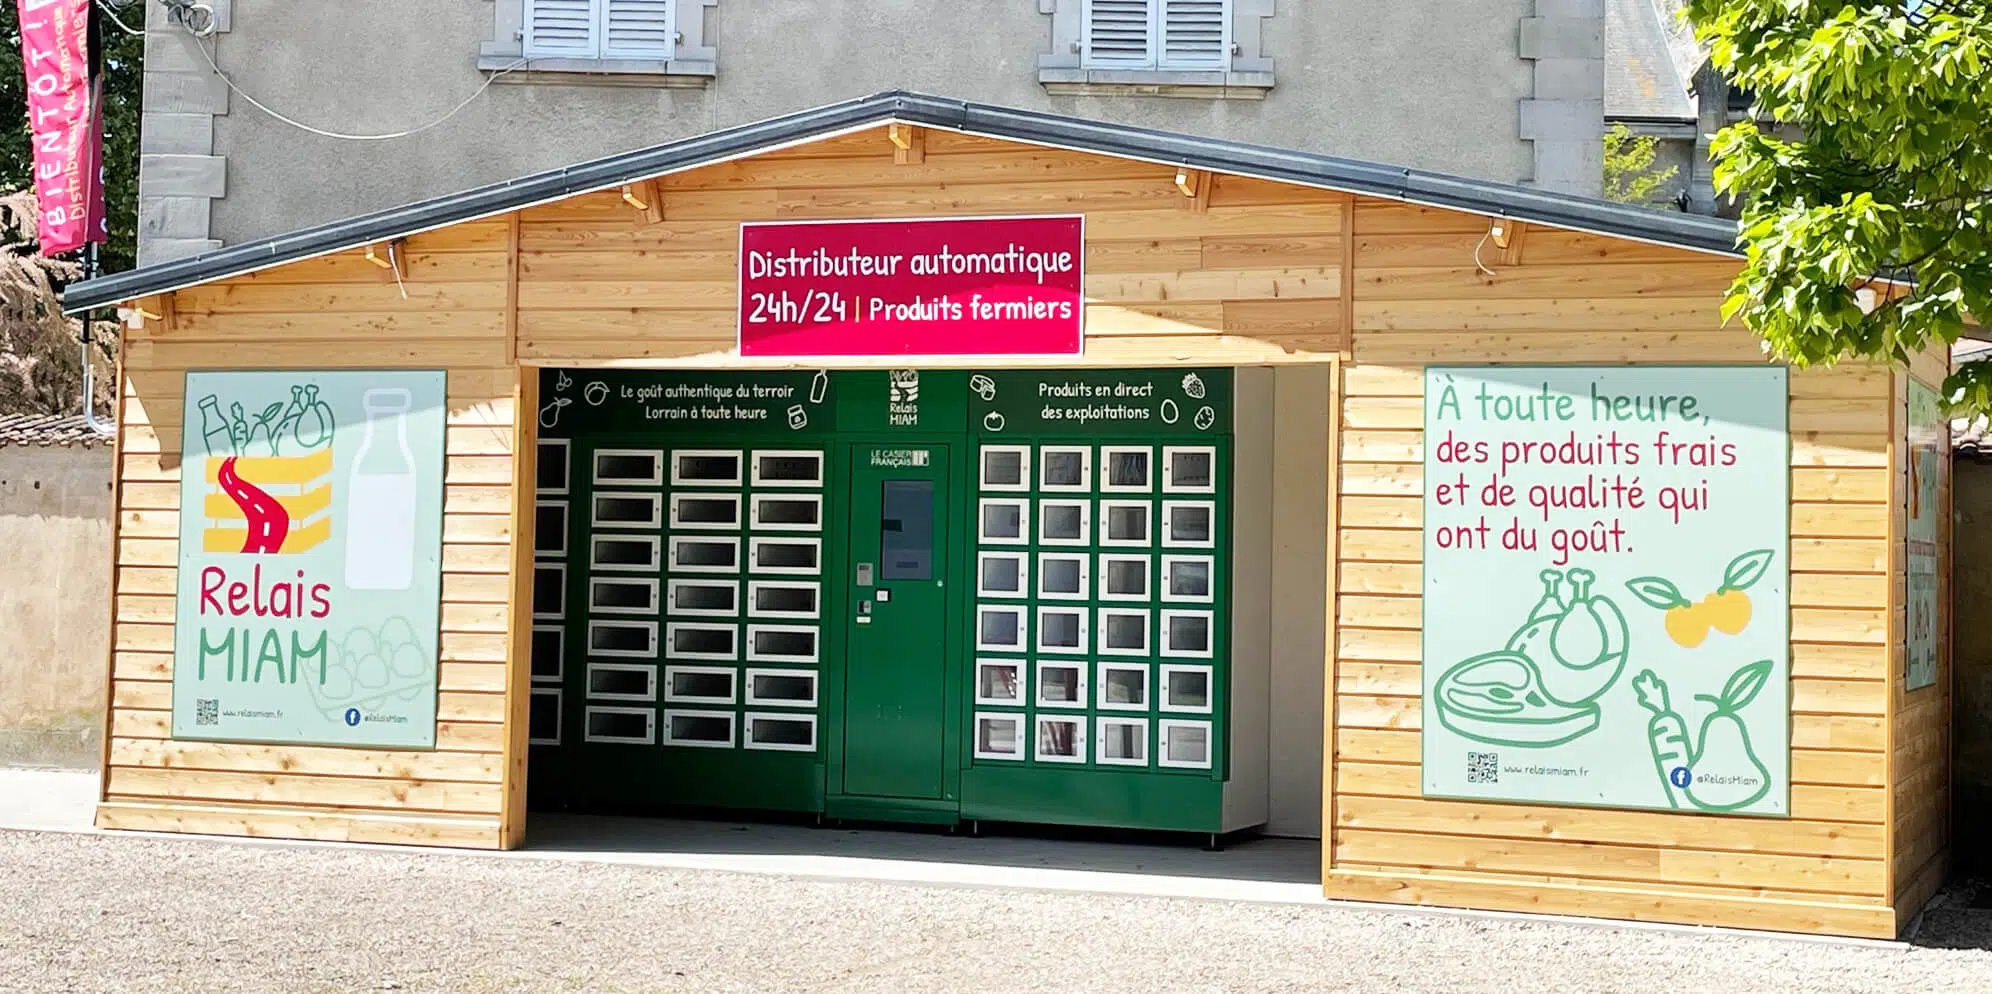
\includegraphics[scale=0.17]{distributeur-produits-fermiers-flirey-54470.jpg}

Distributeur en libre-service de produits fermiers à Flirey en Lorraine
\end{center}

Ce procédé respecte parfaitement le principe de circuit court. En effet, même si le producteur ne rencontre pas directement le client, il n'existe aucun intervenant intermédiaire entre la production et la vente. Ce moyen de vente séduit donc de plus en plus de client et de nouveaux casiers s'implantent alors régulièrement. De plus en plus de sociétés proposent aux producteurs la mise en place de ces casiers. On peut mentionner Nature O Frais qui est aujourd'hui leader en France avec des casiers présents dans 13 départements. De plus, les produits proposés se sont grandement diversifiés. A l'origine, les casiers contenaient exclusivement des fruits et légumes, alors qu'il est désormais possible d'y trouver des oeufs, des yaourts, des jus, du foie gras, des fruits de mer, etc.

\subsection{La solution Locavor}

\hspace{-0.6cm}\begin{minipage}{.7\textwidth}\parindent17pt
C’est un site qui permet de commander des produits locaux, frais et de saison. Le concept du site repose sur les locavores : des points relais gérés par des particuliers ou des professionnels. Le gérant d’un locavore sélectionne les producteurs et organise les ventes avec les produits disponibles sur le site où les clients peuvent mettre au point leur panier. Une date est fixée par le gérant et les clients viennent récupérer leur panier au point relais le plus proche de chez eux. Le site locavore offre la possibilité à chacun de devenir un \og acteur local\fg, avec plus de 170 locavores actifs dans toute la France. 
\end{minipage}%
\hfill
\begin{minipage}{.35\textwidth}%

\includegraphics[width=\textwidth]{locavor_logo.png}
\end{minipage}



\subsection{Mon Panier Local – 06}

\hspace{-0.6cm}\begin{minipage}{.68\textwidth}\parindent17pt


 L’entreprise Mon Panier Local – 06, MPL 06, propose la livraison à domicile sur le département des Alpes-Maritimes d’un panier/cagette de fruits et légumes locaux. Chaque semaine, le client peut commander un panier de fruits et légumes de saison issu de l’agriculture de MLP et complétés par des producteurs locaux. Un panier tel que celui-ci coute 22\euro. Il peut aussi choisir de rajouter d’autres produits selon la disponibilité. 

\end{minipage}%
\hfill
\begin{minipage}{.25\textwidth}%

\includegraphics[scale=0.7]{mpl06.jpeg}
\end{minipage}


\begin{center}
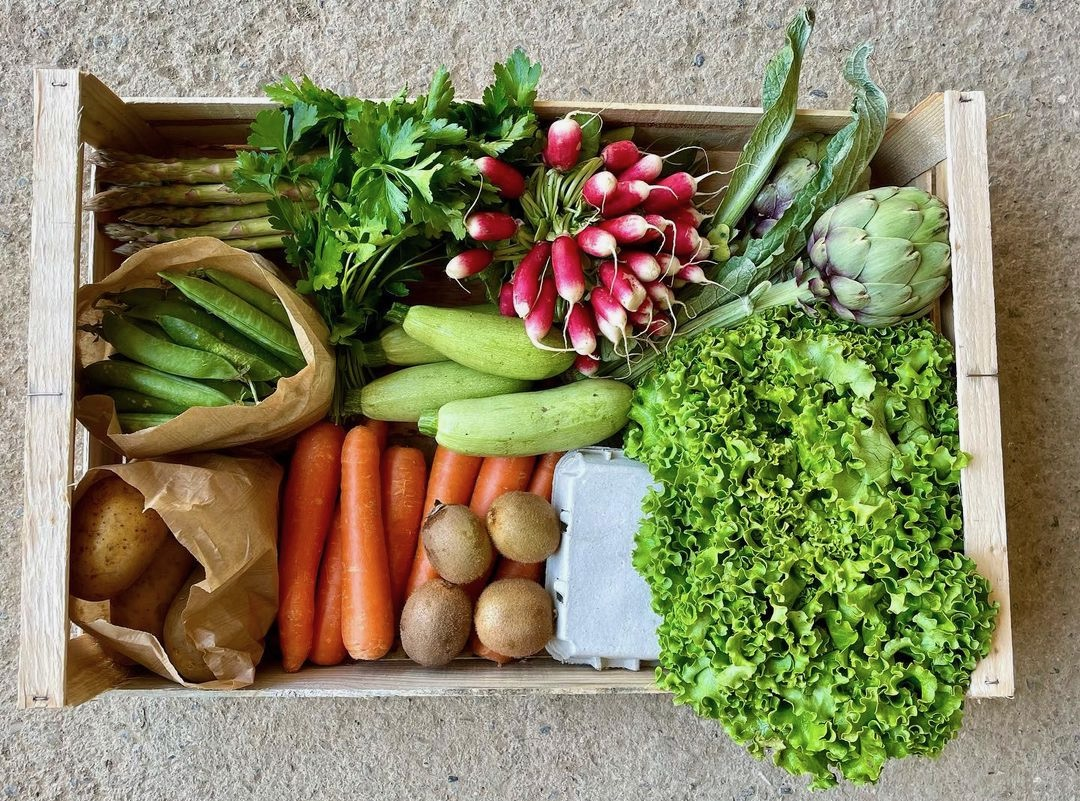
\includegraphics[scale=0.15]{panier.jpeg}
\end{center}

\vspace{0.1cm}

MPL communique la disponibilité des fruits et légumes par mail et gère les commandes par ce biais. Les comptes Facebook et Instagram permettent aux clients de suivre les récoltes et les plantations.  
 
Un mail personnalisé pour le client est envoyé chaque semaine.  


\subsection{Court-circuit à Nancy}

\hspace{-0.6cm}\begin{minipage}{.8\textwidth}\parindent17pt

C’est une épicerie et un café dans le centre ville de Nancy. Partenaire de 30 producteurs locaux, Court-Circuit propose à ses clients d’acheter local, en vrac (limite les emballages) et bio. Il est également possible d’acheter les produits sur la boutique en ligne (en développement) avec un système de click  \& collect. Le seul point de récupération des commandes est à l'épicerie, et il n’est pas encore possible de payer en ligne.


\end{minipage}
\hfill
\hspace{0.5cm}\begin{minipage}{.35\textwidth}%

\includegraphics[scale=0.7]{cc_logo.png}
\end{minipage}
\vspace{0.2cm}

C’est plus qu’un simple supermarché qui ne sélectionne que des produits locaux puisque l’organisation offre des expositions, des rencontres avec les producteurs, des ateliers 0 déchet et d’autres initiatives qui en fait un acteur local important. 


\section{Présentation du concept de l'application} 
\subsection{Le concept}

Notre objectif est de créer une application mettant en relation des particuliers produisant des fruits et légumes en nombre trop important pour leur consommation personnelle avec des acheteurs intéressés par la consommation de produits locaux.

\vspace{0.2cm}

L’exemple d’applications basées sur le circuit court comme Court-Circuit à Nancy montre que ce genre de démarche attire des clients. Cependant, elle emploie une méthode basées sur une unique boutique ce qui ne permet pas de généraliser ce procédé à l’échelle nationale. Plutôt qu’une boutique, notre application utilise des \og cabanes \fg disposées stratégiquement contenant des casiers servant de point-relais entre les 2 parties. 

\subsection{L'interface}

L’interface de l’application contient deux parties distinctes :

\begin{itemize}

\vspace{0.2cm}

	\item Un côté producteur contenant le profil du producteur, la possibilité de mettre en ligne des annonces et de voir l’historique de ses annonces. Il dispose également d’un tutoriel pour aider le producteur à utiliser l’application, ainsi que de le guider vers le casier dans lequel il doit déposer ses produits. Ils ont également la possibilité de poster des images de leurs produits et de leurs espaces de production, afin de se mettre en avant. 

	\item Un côté acheteur ouvrant sur un fil d’offres semblables à un réseau social. Comme les producteurs, chaque acheteur possède un profil. Ces recommandations seront faites selon les récents achats de l’utilisateur, ainsi que de sa localisation (présente les offres les plus proches en premier) à l’aide de filtres. Les différentes offres contiennent le type de produit vendu, le profil du producteur et des recettes associées au produit mis en vente.
	
\end{itemize}

\subsection{Fonctionnalités et contraintes}

Il est également possible de donner un retour sur les produits achetés et d’interagir avec les producteurs via leurs posts. Les commentaires et les notes apparaissent dans le profil du producteur, lui permettant de gagner en visibilité.

\vspace{0.2cm}

Nous nous imposerons de créer une application qui se veut accessible au plus grand nombre, y compris aux personnes peu familières avec l’informatique ou avec les circuits-courts. Cela se traduira par une interface simple, avec des fonctionnalités clairement indiquées.

\subsection{Maquette de l'application}

\begin{center}
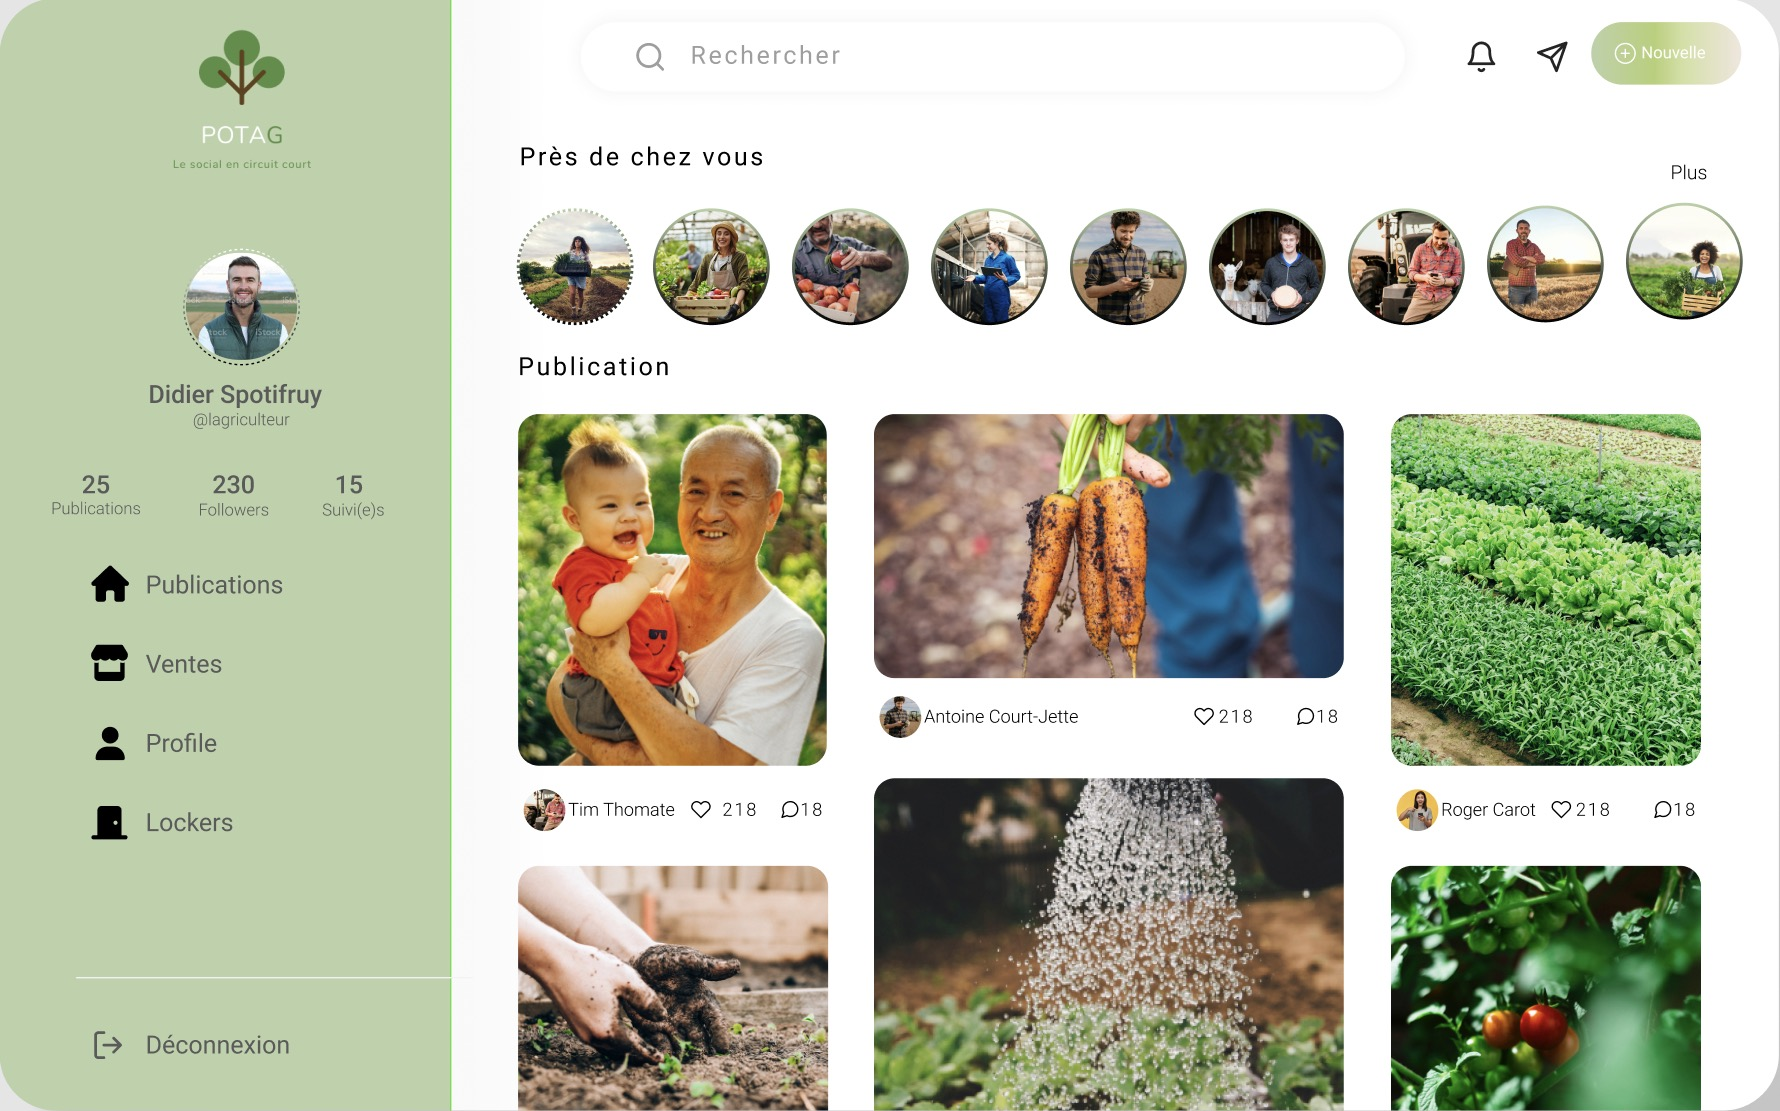
\includegraphics[scale=0.2]{maquette.jpeg}
\end{center}

\section{Gestion de projet}

\subsection{Cahier des charges fonctionnel}

\subsubsection{Principales parties de ce cahier des charges}
\begin{itemize} 
\item Groupe d’expression du besoin et suivi des révisions/validations
\item Présentation générale
\item Expression détaillée du besoin
\item Phases du cycle de vie et environnement
\item Liste des fonctions/services attendus
\item Informations complémentaires
\item Planning
\item Budget
\item Points de vigilance
\end{itemize}

\subsubsection{Auteurs de ce cahier des charges / groupe d’expression du besoin}
\begin{center}
	\begin{tabular}{|l|l|}
	\hline
		\textbf{Nom / email}	& \textbf{Qualité / rôle}\\
		\hline
Maxence BEKHEDDA / maxence.bekhedda@telecomnancy.eu&
Membre de l’équipe projet\\
\hline
Léo GERMAIN / leo.germain@telecomnancy.eu&
Membre de l’équipe projet\\
\hline
Thomas GIANELLI / thomas.gianelli@telecomnancy.eu&
Membre de l’équipe projet\\
\hline
Théo WALTER / theo.walter@telecomnancy.eu&
Membre de l’équipe projet\\
\hline
\makecell[l]{
Olivier FESTOR / olivier.festor@telecomnancy.eu\\
Anne-Claire HEURTEL / anne-claire@telecomnancy.eu\\
Gérald OSTER / gerald.oster@telecomnancy.eu}&
Commanditaires\\
\hline
	\end{tabular}
\end{center}






\subsubsection{Historique des modifications et révisions de ce document}
\begin{center}
	\begin{tabular}{|c|c|c|}
	\hline
		\textbf{n° de version} &	\textbf{Date}	&\textbf{Description et circonstances de la modification}\\
		\hline
V1&	19/10/2022&	1ère version du cahier des charges en vue de la 1ère soutenance\\
\hline
	\end{tabular}
\end{center}


\subsubsection{Résultats et changements attendus}
	Panorama des attendus:
	\begin{itemize}
		\item 	livrables “hard” : aucun
		\item	livrables “soft” : rapport, présentation, application web et le code associé
		\item	livrables “services” : aucun
	\end{itemize}
	
\subsubsection{Parties prenantes}
L'objectif de cette partie est de recenser exhaustivement tous les acteurs concernés par le projet et ses conséquences. On veillera à inclure dans le groupe d’expression du besoin qui rédige ce cahier des charges des représentants 
\vspace{0.2cm}

\noindent Commanditaires: 
\begin{itemize}
	\item 
	initiateurs du projet : Olivier FESTOR, Anne-Claire HEURTEL, Gérald OSTER 
	\end{itemize}
	
\vspace{0.2cm}

\noindent Équipe de réalisation:
\begin{itemize}
	\item Maxence BEKHEDDA
	\item Léo GERMAIN
	\item Thomas GIANELLI
	\item Théo WALTER
\end{itemize}

\vspace{0.2cm}

\noindent Autres parties prenantes :
\begin{itemize}
	\item utilisateur finaux : particulier souhaitant vendre ses fruits et légumes en circuit-court, toute personne souhaitant acheter des fruits et légumes produit par des particuliers à proximité.
		\item	soutiens et opposants au projet : les autres groupes formés d’élèves de 1A créant des applications web répondant au même besoin
		\item	personnes-ressources et experts : Christophe BOUTHIER, Olivier FESTOR, Anne-Claire HEURTEL, Gérald OSTER 
\end{itemize}


\subsubsection{Contraintes de planning}
\begin{itemize}
	\item 	1er rapport : 20/10/2022 à 18h
		\item	1ère soutenance : 22/10/2022 à 9h
		\item	Date de rendu du projet : 06/01/2023
		\item	Date de soutenance : 14/01/2023
\end{itemize}

\newpage
\subsection{To-Do List en vue de la première soutenance}

\rotatebox{90}{
	\begin{tabular}{|c|c|c|c|c|c|c|c|}
\hline
	\textbf{Tâches} & 
		\makecell[c]{\textbf{Priorité}\\
		\textbf{(0-4)} \\}& 
		\makecell[c]{\textbf{Date} \\\textbf{de} \\\textbf{début} }& 
		\makecell[c]{\textbf{Date} \\\textbf{de}\\ \textbf{fin}} &
		\makecell[c]{\textbf{Charge}\\ \textbf{de}\\ \textbf{travail}} & 
		\textbf{Livrables} & 
		\textbf{Progrès} & 
		\makecell[c]{\textbf{Dernière} \\\textbf{mise à}\\ \textbf{jour}}\\
		\hline
		État de l'art&
		4&
		10/10/22&
		18/10/22&
		8h&
		\makecell[c]{
		Chercher et relever quelques exemples\\ d’applications web de vente de fruits et\\ légumes en circuit court existantes afin \\de les mettre en perspective avec notre \\application}&
		100\%&
		17/10/22\\
		\hline
		\makecell[c]{Gérer la gestion\\ du projet}&
		2&
		10/10/22&
		18/10/22&
		6h&
		\makecell[c]{Rédiger des comptes-rendus pour chaque\\ réunion. Définir la démarche avec une \\to-do list et un cahier des charges.}&
		100\%&
		17/10/22\\
		\hline
		\makecell[c]{Expliquer le concept\\ de l'application et \\ son aspect innovant}&
		2&
		14/10/22&
		18/10/22&
		2h&
		\makecell[c]{Expliquer avec détails le concept de \\l’application. Puis, à partir de l’état de \\l’art, énoncer ses caractéristiques \\innovantes.}&
		100\%&
		17/10/22\\
		\hline
		Rédiger le rapport&
		2&
		16/10/22&
		18/10/22&
		8h&
		\makecell[c]{Rédiger un rapport détaillé reprenant \\tous les points majeurs attendus de \\notre démarche : \\
\hspace*{-1cm}-\;	L’état de l’art\\
\hspace*{0.1cm}-\;	La gestion du projet\\
\hspace*{0.8cm}-\;	L’explication du concept
}&
		80\%&
		17/10/22\\
		\hline
		\makecell[c]{Réaliser la \\ présentation}&
		2&
		16/10/22&
		18/10/22&
		4h&
		Créer un support de présentation concis&
		60&
		17/10/22\\
		\hline
		\makecell[c]{Préparation finale\\ en vu de la \\soutenance}&
		2&
		16/10/22&
		18/10/22&
		2h&
		\makecell[c]{Organisation des temps de parole et \\préparatifs en vue de la soutenance}&
		50\%&
		17/10/22\\
		\hline
	\end{tabular}
}	

\newpage


\subsection{Compte rendu de la première réunion}

\begin{center}

\begin{tabular}{|p{8.3cm}|p{8.3cm}|}
\hline

	 Motif / type de réunion: Réunion technique &  
	 Lieu: Telecom Nancy (0.09)\\
	 
	\hline 
	
	Présent(s) (retard/excusés/non excusés):&
	Date / heure de début / durée:\\
	
	\makecell[lll]{
	Équipe-projet : &
 BEKHEDDA Maxence \\
& GERMAIN Léo \\
& GIANELLI Thomas \\
& WALTER Théo}&
	\makecell[l]{
10/10/2022 à 13h\\
Durée : 1h}\\
\hline

\end{tabular}

\end{center}


\subsubsection{Ordre du jour}

\begin{enumerate}

	\item 
	Retour sur les attendus du projet, en reprenant point par point l’énoncé.
\item 	Mise en commun des premières idées ainsi que des recherches préliminaires sur l’état de l’art, travaillés au préalable.
\item 	Répartition des objectifs

\end{enumerate}

\vspace{0.5cm}

\subsubsection{Informations échangées}
\vspace{0.2cm}

	Idée de sujet : Mettre les producteurs en relation avec de potentiels acheteurs à proximité via une application web. Mettre en place des « cabanes » contenant des casiers réfrigérés dans lesquels les acteurs pourraient déposer leurs fruits et légumes, suivant le modèle des points-relais d’Amazon. Les acheteurs pourraient ensuite venir dans ces cabanes acheter les produits. Les stocks, l’historique des ventes et des informations sur les acheteurs et les vendeurs seraient contenues dans des bases de données.

\vspace{0.5cm}

\subsubsection{Remarques / Questions}
\vspace{0.2cm}

\begin{itemize}
	\item Question 1 : Est-ce suffisant pour inclure tous les domaines étudiés en CS54, requis pour le projet ?
	\item Question 2 : Nous avons peu de temps avant la première présentation. Comment nous répartissons-nous les tâches ?

\end{itemize}

\vspace{0.5cm}
\subsubsection{Décisions} 
\vspace{0.2cm}

\begin{itemize}
	\item 

	Réponse 1 : Idée additionnelle : Mettre en place deux interfaces producteur/acheteur. L’interface acheteur, semblable à un fil d’actualité de réseau social propose des produits suivant le profil de l’acheteur. Des filtres et des suggestions seraient gérées par un algorithme. L’interface producteur, plus simple, permettrait au producteur d’indiquer le type de produits qu’il souhaite vendre, et lui indiquer l’endroit où il peut les déposer. Cela permet d’inclure l’algorithmique et la programmation web.

\item	Réponse 2 : Une personne s’occupera du lien avec la gestion de projet. Les trois autres personnes s’occuperont d’approfondir l’état de l’art, en séparant l’échelle locale et l’échelle globale.
\item	Décision 3 : A la prochaine réunion, nous devons d’abord mettre en commun nos avancées. Puis, nous allons échanger des idées et se répartir des objectifs concernant la création de la présentation, et la description du concept de l’application et son innovation.

\end{itemize}
\vspace{0.5cm}

\subsubsection{Actions à suivre / Todo list}
\vspace{0.2cm}

\begin{center}
\begin{tabular}{|p{4cm}|p{4cm}|p{1cm}|p{3cm}|p{2cm}|}
\hline
\centering Description & 
\centering Responsable & 
\centering Délai & 
\centering Livrable & 
\hspace{0.05cm} Validé par\\
\hline
État de l'art (Nancy et ses environs) & WALTER Théo & 16/10 & Présentation & L'équipe projet \\
\hline
État de l'art (à l'échelle globale) & BEKHEDDA Maxence GIANELLI Thomas & 16/10 & Présentation & L'équipe projet\\
\hline
Gestion du projet & GERMAIN Léo & 16/10 & Compte-rendu, Matrice SWOT & L'équipe projet \\
\hline
	
\end{tabular}
\end{center}

\subsection{Compte rendu de la deuxième réunion}

\begin{center}

\begin{tabular}{|p{8.3cm}|p{8.3cm}|}
\hline

	 Motif / type de réunion: Stand-up Meeting &  
	 Lieu: Telecom Nancy (0.09)\\
	 
	\hline 
	
	Présent(s) (retard/excusés/non excusés):&
	Date / heure de début / durée:\\
	
	\makecell[lll]{
	Équipe-projet : &
 BEKHEDDA Maxence \\
& GERMAIN Léo \\
& GIANELLI Thomas \\
& WALTER Théo}&
	\makecell[l]{
15/10/2022 à 12h\\
Durée : 10min}\\
\hline

\end{tabular}

\end{center}

\subsubsection{Ordre du jour}

\begin{enumerate}

	\item 
		Retour sur le travail effectué par chacun depuis la dernière réunion.
\item 	Difficultés rencontrées/Nouvelles idées.
\item 	Listing et répartition des tâches restantes.

\end{enumerate}

\vspace{0.5cm}

\subsubsection{Informations échangées}
\vspace{0.2cm}

\begin{itemize}
	\item 	Nous avons avancé sur l’état de l’art. L’idée d’utiliser des casiers comme points-relais pour la vente de fruits et légumes dans des endroits stratégiques existe déjà. Cependant, l’aspect social que nous ajoutons dans l’application via les algorithmes de recommandation est innovant. Nous pourrions de plus ajouter dans l’application des liens vers des recettes concernant les fruits et légumes achetés, ou encore les emplacements de composts collectifs à proximité permettraient d’agir en circuit court tout le long de la vie du produit : production, vente, consommation, recyclage.
	\item 	Les étapes suivantes sont : rédiger la description complète de l’application et son aspect innovant et préparer la soutenance : répartition des temps de parole, support de présentation.
	\item La partie de gestion de projet est complétée au fur et à mesure, avec les comptes-rendus de réunion, et avec les connaissances apportées au fur et à mesure par le MOOC. Par exemple, nous savons à présent qu’il est nécessaire d’effectuer une charte de projet.
\end{itemize}

\vspace{0.5cm}

\subsubsection{Remarques / Questions}
\vspace{0.2cm}

\begin{itemize}
	\item Question 1 :Comment nous répartissons-nous les tâches ?	
	\item Question 2 : Dans quelle mesure allons-nous utiliser le LaTeX et savons-nous utiliser LaTeX ?
	\item Quel sera l’ordre du jour de la prochaine réunion ?

\end{itemize}

\vspace{0.5cm}
\subsubsection{Décisions} 
\vspace{0.2cm}

\begin{itemize}
	\item 

	Réponse 1 : Nous allons nous répartir en deux binômes. L’un s’occupe de la préparation de la soutenance. L’autre se charge de la rédaction du concept de l’application et de son innovation. Chacun peut également poursuivre ses recherches sur son objectif précédent pour compléter son rapport si nécessaire.
\item	Réponse 2 : 3 des 4 membres savent utiliser LaTeX. Nous allons convertir les différents documents dont les comptes-rendus en LaTeX. Cependant, le support de présentation ne sera probablement pas en LaTeX.
\item	Décision 3 : La prochaine réunion sera sûrement la dernière avant le rendu du livrable (le support de présentation) prévue le 20/10/2022. Il faudra donc le présenter à l’intégralité de l’équipe projet et noter toutes les remarques afin d’avoir la version finale au plus vite. Pour cela, la partie explication du concept et de l’aspect innovant de l’application doit également être complet et validé par l’équipe projet.

\end{itemize}
\vspace{0.5cm}


\subsubsection{Actions à suivre / Todo list}
\vspace{0.2cm}

\begin{center}
\begin{tabular}{|p{4cm}|p{4cm}|p{1cm}|p{3cm}|p{2cm}|}
\hline
\centering Description & 
\centering Responsable & 
\centering Délai & 
\centering Livrable & 
\hspace{0.05cm} Validé par\\
\hline
Préparation de la soutenance (support de présentation) & WALTER Théo \newline GERMAIN Léo & 18/10 & Présentation du support& L'équipe projet \\
\hline
Explication du concept de l'application et de son aspect innovant & BEKHEDDA Maxence GIANELLI Thomas & 18/10 & Présentation d'un rapport & L'équipe projet\\
\hline

	
\end{tabular}
\end{center}

\newpage
\nocite{*}
\bibliographystyle{plain}
\bibliography{biblio}

\end{document}

